%----------------------------------------------------------------------------------------
% METADATA BLOCK (YAML)  — see inbox/README.md
%----------------------------------------------------------------------------------------
% uid: ""
% school: "lycee"
% level: "2eme"
% section: ["Sciences", "Informatique"]
% chapter: "Barycentre"
% title: "Barycentres dans un repère"
% difficulty: "Facile"
% tags: ["barycentre", "coordonnees", "barycentre-partiel", "milieu"]
% provenance: "own"
% batch: "2026-11-19-2sc-polynomes-barycentre"
%----------------------------------------------------------------------------------------

\newcommand{\R}{\mathbb{R}}
\newcommand{\vect}[1]{\overrightarrow{#1}}

% ---STATEMENT---
Le plan est muni d'un repère $(O,\vec i,\vec j)$. On donne $A(-1\,;3)$, $B(3\,;1)$ et $C(1\,;-3)$.
\begin{enumerate}
  \item Calculer les coordonnées du point $G$, barycentre de $(A,1)$ et $(B,3)$.
  \item Montrer que le point $E(5\,;0)$ est le barycentre de $(A,-1)$ et $(B,3)$.
  \item Calculer les coordonnées du point $K$, barycentre de $(A,1)$, $(B,3)$ et $(C,4)$.
  \item Montrer de deux façons que $K$ est le milieu du segment $[GC]$ : par les coordonnées, puis avec le barycentre partiel.
\end{enumerate}

% ---SOLUTION---
\begin{center}
% alt: Repère avec les points A, B, C, G, E, K ; G et E sur la droite (AB), K milieu de [GC].
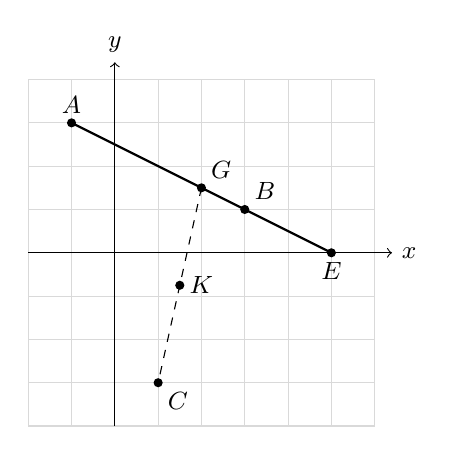
\begin{tikzpicture}[scale=0.55, font=\small]
  \draw[gray!30] (-2,-4) grid (6,4);
  \draw[->] (-2,0)--(6.4,0) node[right]{$x$};
  \draw[->] (0,-4)--(0,4.4) node[above]{$y$};
  \draw[thick] (-1,3)--(5,0);
  \draw[dashed] (2,1.5)--(1,-3);
  \foreach \p/\x/\y/\pos in {A/-1/3/above, B/3/1/above right, C/1/-3/below right, G/2/1.5/above right, E/5/0/below, K/1.5/-0.75/right}
    {\fill (\x,\y) circle (3pt) node[\pos] {$\p$};}
\end{tikzpicture}
\end{center}
\begin{prop}[Coordonnées du barycentre]
Si $G$ est le barycentre de $(A,\alpha)$, $(B,\beta)$, $(C,\gamma)$ avec $\alpha+\beta+\gamma\neq0$, alors
\ib{$x_G=\dfrac{\alpha x_A+\beta x_B+\gamma x_C}{\alpha+\beta+\gamma}$} et \ib{$y_G=\dfrac{\alpha y_A+\beta y_B+\gamma y_C}{\alpha+\beta+\gamma}$} (même formule sans $C$ pour deux points).
\end{prop}
\begin{enumerate}[itemsep=14pt]
  \item Somme des coefficients : $1+3=4$.
  \[x_G=\dfrac{1\times(-1)+3\times3}{4}=\dfrac84=2\qquad y_G=\dfrac{1\times3+3\times1}{4}=\dfrac64=\dfrac32\qquad G\left(2\,;\dfrac32\right)\]

  \item Somme des coefficients : $-1+3=2\neq0$, le barycentre existe. On calcule ses coordonnées :
  \[x=\dfrac{(-1)\times(-1)+3\times3}{2}=\dfrac{10}{2}=5\qquad y=\dfrac{(-1)\times3+3\times1}{2}=\dfrac02=0\]
  On retrouve $(5\,;0)$ : $E$ est bien le barycentre de $(A,-1)$ et $(B,3)$.

  \item Somme des coefficients : $1+3+4=8$.
  \[x_K=\dfrac{-1+9+4}{8}=\dfrac{12}{8}=\dfrac32\qquad y_K=\dfrac{3+3-12}{8}=-\dfrac68=-\dfrac34\qquad K\left(\dfrac32\,;-\dfrac34\right)\]

  \item \textbf{Méthode 1 (coordonnées).} Le milieu de $[GC]$ a pour coordonnées
  \[\left(\dfrac{2+1}{2}\,;\dfrac{\frac32-3}{2}\right)=\left(\dfrac32\,;-\dfrac34\right)\]
  Ce sont les coordonnées de $K$.

  \textbf{Méthode 2 (barycentre partiel).}
  \begin{prop}[Associativité]
  Dans un système de points pondérés, on peut \ib{remplacer deux points par leur barycentre}, affecté de la somme de leurs coefficients (si elle est non nulle).
  \end{prop}
  $G$ est le barycentre de $(A,1)$ et $(B,3)$ : on remplace ces deux points par $(G,4)$.

  Donc $K$ est le barycentre de $(G,4)$ et $(C,4)$ : deux coefficients égaux, $K$ est le milieu de $[GC]$.
\end{enumerate}
